\documentclass[preprint]{aastex62}

% \usepackage{minted}
\usepackage{amsmath}
\usepackage{listings}
\usepackage{courier}
\usepackage{cleveref}
\usepackage{float}

\definecolor{bcolor}{RGB}{0, 51, 153}
\definecolor{gcolor}{RGB}{51, 153, 51}

\shorttitle{photon counting \& detectors}
\shortauthors{j. birky}

\begin{document}

\title{\sc Lab 1: Photon Counting \& Detectors}
\author{Jessica Birky, Julian Beaz-Gonzalez, Russell Van-Linge}

\correspondingauthor{Jessica Birky (A13002163)}
\email{jbirky@ucsd.edu}

\begin{abstract}
In this lab, we examine the statistics of photon counting, and the noise properties of a charged couple device (CCD) from $2048\times2048$ pixel optical images taken on the Nickel 1 meter direct imaging camera. In particular we characterize the effect of several types of noise: first the inherent noise of photon counting by comparing to the Poisson distribution, second the read noise associated with random charge loss and gains, and lastly we comment the effect of different systematics such as instrument defects or dark current due to temperature variations. In total we collect 22 frames integrated at varying exposure times ranging from 0 to 768 seconds. Comparing the slope and intercept between mean and variance of each bias-subtracted, combined frame of each exposure, we determine the gain of the detector to be 0.31 ADU/electron and the readnoise to be 34 electron. Normalizing our frames (dividing the counts by exposure time) we find that as we add more exposures, the mean of the mean (MOM) detector counts per second converges to 50.2 ADU/s and the standard deviation of the mean (SDOM) decreases to 34.2 ADU/s with more frames added.

\end{abstract}
\bigskip

\section{Introduction} 
Nearly the only way to study the Universe on the largest of scales (such as stars and galaxies), and probe into the 12 to 14 billion years of our Universe's history (such as detecting cosmic microwave background from the early Universe) requires measuring information in the form of light, traveling at $3\times10^8$ m/s. Advancements in technology in the 20th century has now made it possible to observe electromagnetic radiation from the scales of $10^{-12}-10^3$m (as short as gamma rays to as long as radio waves), far beyond the optical range accessible to our eyes using telescopes of previous times. Because the measurement of light is so fundamental, understanding how modern detectors measure electromagnetic radiation, the statistics of photon collection, as well as the limitations of the instrument and sources of contaminations are a important first steps before performing any scientific analysis of light with an instrument.

Three types of detectors in astronomy measure light using different approaches: coherent detectors measure the amplitude and phase of the electric field produced by an electromagnetic wave, calorimetric detectors measure the heat produced from radiation, and photoelectron detectors indirectly measure photons by counting electrons which are produced by the photoelectric effect when light excites electrons on a piece of semiconductor. In particular, this lab seeks to understand how photoelectric detectors called charged coupled device (CCD) detectors work for collecting photons at optical wavelengths.

As we'll see in later sections, there are several sources of noise associated with CCDs that are important to classify: (1) the Photon noise associated with Poisson statistics, (2) the bias level noise associated with electronic variation which varies pixel-to-pixel, (3) readnoise associated with random fluctuations of charge loss/gains when electrons are shuffled between detector pixels to be readout, (4) the dark current noise from the heat of the detector which may cause more electrons to excite for higher temperatures, and (5) any systematics like defects in the detector. Section \ref{sec:methods} covers how we quantify these sources of noise, and Section \ref{sec:analysis} shows what values we compute for data taken on the Nickel Observatory described in Section \ref{sec:observations}. 

% ==================================
\section{Observations} \label{sec:observations}
Observations are taken on the Nickel 1 meter telescope, Lick Observatory located on Mount Hamilton. We recorded 22 frames in total (Table \ref{table:log}) using the B filter, corresponding to the optical wavelengths $3,500-5,000$ Angstroms\footnote{https://mthamilton.ucolick.org/techdocs/filters/B\_plot.html}. Frames are labeled as either `Bias' (open shutter for zero second exposure), or `Flat' (several second exposure).

\begin{table}[H]
\centering
\begin{tabular}{|c|c|c|c|c|}
    \hline
    Start File \# & End File \# & \# Frames & Type  & Exposure Time (sec) \\
    \hline
    \hline
    401 & 404 & 5 & Bias & 0  \\
    420 & 421 & 2 & Flat & 3 \\
    422 & 425 & 4 & Flat & 6 \\
    426 & 428 & 3 & Flat & 12 \\
    429 & 431 & 3 & Flat & 24 \\
    432 & 434 & 3 & Flat & 48 \\
    435 & 437 & 3 & Flat & 96 \\
    438 & 439 & 2 & Flat & 192 \\
    440 & --  & 1 & Flat & 384 \\
    441 & --  & 1 & Flat & 768 \\
    \hline
\end{tabular}
\caption{Observation log, recording the files associated with each exposure time. Files $405-418$ were removed due to inconsistent count numbers.} \label{table:log}
\end{table}


% ==================================
\section{Data Reduction \& Methods} \label{sec:methods}
\subsection{Theoretical Distribution of Light} \label{subsec:distributions}
Before we can characterize our observations, it is important to first determine what we expect our data will look like. That is, we are measuring the number of photons hitting a detector over a fixed amount of time, what do we predict will be the number of photons that will hit each pixel in that tme interval? Let's assume that on average $\mu$ photons will hit a pixel over fixed time interval $t$. Now consider dividing that time interval into $n$ increments: the probability that a $n$ photons arrive to the detector is approximately Binomial with probability parameter $\mu/n$. Now in the limit that $n\rightarrow\infty$, we come to the Poisson distribution:
\begin{equation}
P(x;\mu) = \frac{\mu^x}{x!}e^{-\mu}
\end{equation}
which we interpret as the probability that x photons will arrive to a detector pixel in time interval $t$, given that $\mu$ photons arrive in that interval on average. The expected mean and variation for this distribution being $\langle x \rangle = \mu$ and $\langle \sigma^2 \rangle = \mu$. 

In practice, the Poisson distribution is unstable to compute for large values of x because the term $x!$ becomes too large for the memory of the computer to handle. In order to try to reduce the memory load for large values of x, we approximate the $x!$ term using the Sterling approximation:
\begin{equation}
n! \sim \sqrt{2\pi n}\left(\frac{n}{e} \right)^n
\end{equation}
the code for the Poisson distribution is implemented in lines $7-9$ of Appendix \ref{code:stats}.

However when the conditions for the Poisson distribution are not met very well (average number of successes is much smaller than the probable value ($\mu << n$), and the number of counts are low), the Gaussian distribution may instead be a good approximation:
\begin{equation}
P(x; \mu, \sigma) = \frac{1}{\sqrt{2\pi}} e^{-\frac{(x-\mu)^2}{2\sigma^2}}
\end{equation}
where the input parameters are the mean and standard deviation of the data ($\mu$ and $\sigma$). The code for the Gaussian distribution is implemented in lines $11-13$ of Appendix \ref{code:stats}. 

\subsection{Data Reduction} \label{sec:reduction}
For each exposure observed, the data output from the Nickel instrument is stored in a fits file, which contains the two-dimensional array of detector counts at each pixel, as well as other relevant variables about the detection (such as the detector temperature, time of observation, exposure time, etc.). The first step of reduction consists of combining the bias frames, and our procedure for combining frames (lines $19-26$, \ref{code:data}) is to take the median count value at each pixel. Second, for each exposure, we read the individual files from a directory, subtract the combined bias, then combine those into a single frame (lines $9-11$, \ref{code:reduction}).

As discussed in further the results (\ref{subsec:systematics}), large chunks of the $2048\times2048$ pixel image contain detector defects and contaminations which skew the distribution of light counts. In order to reduce these effects, we slice our image to a $15\times15$ pixel section chosen from the longest exposure time image (Figure \ref{fig:slice}) before performing bias subtraction.

\subsection{Types of Detector Noise} \label{subsec:noise}
Photons collected by the detector of an instrument are not counted directly--the CCD used by the Nickel telescope relies on the photoelectric effect, meaning that it photons excite electrons on a piece of semiconductor and the charge from those electrons is recorded by an analog to digital converter (ADC) in analog to digital units (ADU; an 8-bit number $0-255$ which can be stored on a computer). In order to reverse this and determine the actual number of photons from ADU counts, we must know how to convert the voltage of the accumulated charge 
\begin{equation}
V = \frac{Q}{C} = \frac{Ne}{C}
\end{equation}
where $e=1.6\times10^{-19}$ is the charge of an electron, $C$ is the capacitance (typically on the order of several picoFarads), and $N$ is the number of electrons into analog digital units. Generally, the ADU count is linearly proportional by constant $g$ to the voltage, with some bias $ADU_0$:
\begin{equation}
ADU = g\frac{Ne}{C} + ADU_0
\end{equation}

Propagating the error (assuming negligable covariance), we get a formula that relates the average number of ADU counts to it's variance:
\begin{align}
\sigma_{ADU}^2 &= \left(\frac{\partial ADU}{\partial N} \right) \sigma_N^2 + 
    \left(\frac{\partial ADU}{\partial \sigma_0} \right) \sigma_0^2 \\
    &= \frac{ge}{C} \left(ADU - ADU_0 \right) + \sigma_0^2
\end{align}
Thus the gain (ge/C) is the linear slope between the mean and variance of the ADU counts for each bias-subtracted, combined exposure frame $\left(ADU - ADU_0 \right)$, and the readnoise is the intercept $\sigma_0$. To numerically determine the gain from our data we fit a second-order polynomial to our mean vs. variance plot (lines $1-7$, \ref{code:gain}), and the gain is then the first order term (coefficient of x).

% ==================================
\section{Data Analysis \& Modeling} \label{sec:analysis}

\subsection{Diagnostic Plots: Combined Images \& Histograms} \label{subsec:diagnostic}
Figure \ref{fig:bias} shows the combined bias frames, and the figures in \ref{fig:flats1} and \ref{fig:flats2} show the bias-subtracted, combined histograms and images for each of the eight different exposure times (3, 6, 12, 24, 48, 96, 192, 384, and 768 seconds), using the procedures described in \ref{sec:reduction}. Lines $25-33$ of \ref{code:plots} plots the histogram, and lines $72-75$ plot the image.

The left side of each panel shows the histogram of the number of detector counts in analog to digital units (ADU), normalized such that the sum of all of the bins is one (plotted in black). The solid blue vertical line marks the mean of the data, and the dashed blue line marks the median, indicating which distrubtions are symmetric or skewed. For all histograms however, the mean and median are very close, meaning the distributions are quite symmetric. The two shades of green mark $\pm1$ and $\pm2$ standard deviations above and below the mean. Finally, the distribution in red shows the expected Poisson distribution, as a function of the mean of the data ($\bar{x}$), with a one standard deviation range also shaded in red (where the expected standard deviation for the Poisson is $\sigma=\sqrt{\bar{x}}$). The distribution in cyan shows the Gausian fit using the mean and standard deviation of the data ($\bar{x}, s$). The Poisson and Gaussian distributions are scaled to the data by first normalizing to one, then multiplying by the max frequency of the data (lines $50-51$ and $58-59$, \ref{code:plots}).

The right side of each panel shows the 2D images. In order to visualize the detector counts per pixel, we must map the number of counts to an RGB color value, which we use the {\tt matplotlib} `gray' colormap for. To emphasize the features in the data, we choose the min an max values of the colormap to be the 10th and 90th percentile counts of the data.

\begin{figure}[H]
\plotone{plots/exposure0.png}
\caption{Combined bias frames.} \label{fig:bias}
\end{figure}

\subsection{Mean of the Mean \& Standard Deviation of the Mean}
For each of our bias-subtracted frames, we divide the arrays by their exposure times to put them on the same scale of counts per second, and we take the means (giving us a $1\times22$ array of the average values for 22 frames). Next we compute the mean of the mean (MOM) and standard deviation of the mean (SDOM) in a for loop (lines $1-37$, \ref{code:mom_sdom}): the first MOM/SDOM are the mean and standard deviation of the first frame taken, the second is the MOM/SDOM for the first two frames, and so on. The resulting plot (Figure \ref{fig:mom_sdom}) shows how the standard deviation decreases with larger N (more number of observations) and the mean stays roughly constant because the normalized distributions are centered around roughly the same peak.

More precisely, the standard deviation decreases by a factor of 1/$\sqrt{N}$. This factor arises because each distribution is approximately Gaussian (as seen in the histogram fits) and they are normalized to the same count, so we can assume we are roughly summing together individual Gaussians with the same mean and standard deviation parameters. If we consider generally $n$ gaussian distributed random numbers $X_1,...,X_i,...,X_n \sim N(\mu,\sigma^2)$, the variance of the sum of the distributions is then
\[Var(\bar{X}) = Var(\frac{1}{N}\sum_{i=1}^N X_i) = \frac{1}{n^2} Var(X_i) = \frac{1}{n^2} \cdot n\sigma^2 \]
since the variance of the Gaussian is linear. Then we get the standard deviation of the sum is just the square root
\[Std(\bar{X}) = \sqrt{Var(\bar{X})} = \frac{\sigma}{\sqrt{n}} \]
meaning as you add more gaussian distributed observations, the SDOM decreases by 1/$\sqrt{n}$.

\begin{figure}[H]
\begin{center}
\includegraphics[width=.48\linewidth]{plots/mom_sdom.png}
\caption{Mean of the mean and standard deviation of the mean vs. number of frames taken (N). In red we show the predicted SDOM, which decreases by factor of 1/$\sqrt{N}$ for each frame added. \textit{Credit: Russell}} \label{fig:mom_sdom}
\end{center}
\end{figure}

\subsection{Quatifying Detector Noise} \label{subsec:gain}
Figure \ref{fig:mean_var} is the mean vs. variance plot for each bias-subtracted, combined exposure. As described in \ref{subsec:noise} we fit a second-order polynomial using {\tt numpy} to the point on the plot. The fit is mostly described by the first-order gain term which is 0.31 ADU/electron, with a very small second-order correction of $4.2\times10^{-5}$ ADU/electron. The intercept (readnoise) of the fit is 34 electrons. Although the fit looks like it represents the data points well, our results deviate from the official specifications listed on the Nickel website\footnote{\footnotesize https://mthamilton.ucolick.org/techdocs/instruments/nickel\_direct/detector/ \\?fbclid=IwAR1jiS4gzq1GNTfHfXq6cv2KNNky70EokCcHCyL6h0spe4YHOJ2VdZsyRSw}, which state the gain is 0.56 ADU/electron and the readnoise is 10.7 electrons.

\begin{figure}[H]
\begin{center}
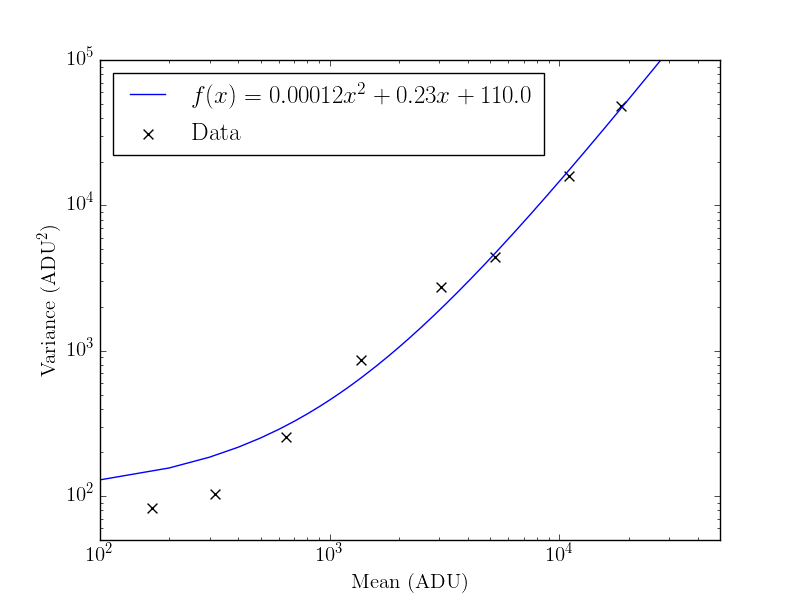
\includegraphics[width=.48\linewidth]{plots/mean_vs_variance.png}
\caption{Mean vs. variance for all bias-subtracted exposures, fitted to a second-order polynomial. First order coefficient represents the gain, intercept represents the readnoise.} \label{fig:mean_var}
\end{center}
\end{figure}

% ==================================
\section{Discussion} \label{sec:discussion}
\subsection{Poisson \& Gaussian Comparisons} \label{subsec:dist_comparisons}
As described in Section \ref{subsec:distributions}, we expect that the Poisson distribution would approximate our data well when $\mu$ is the smallest (the frames with lower exposure times). However, our results in Figures \ref{fig:flats1} and \ref{fig:flats2} show the opposite trend: the Gaussian appears to be a slightly better fit for low exposure times, but the Poisson appears better for higher exposure times.

This discrepancy in trend is likely due to the fact that another condition of the Poisson distribution is that the frequency of counts must also be low. Looking at the y-axis of our histograms, low exposure times show the highest frequency counts (a max of 14 for the 3 second exposure) and the lowest frequency counts for high exposure times (less than 4 for exposures more than 192 seconds). Although we tried minimizing the window slice as much as possible (to $15\times15$ pixels), and looked at different regions on the detector, the trends we see in Figures \ref{fig:flats1} and \ref{fig:flats2} remained pretty much consistent. In any case, we conclude both the Poisson and Gaussian are both pretty good approximations to our data.

\subsection{Sources of Noise \& Systematic Effects} \label{subsec:systematics}
While analyzing our data, we also discovered that there are several different kinds of systematic contaminations which appeared to affect the distributions of counts that we saw. Looking at the full $2048\times2048$ images we found that the detector count distribution was close to a Poisson distribution for low exposure times, but for larger exposure times it increasingly diverges with a much larger standard deviations than expected. We also saw that low exposure times (3, 6, and 12 sec) have a single peak in the distribution around the mean, however at 48 sec the distribution becomes bimodal, and for high exposure times (96, 192, 384, and 768 sec) the distribution develops three separate peaks. Slicing our data to a small region, we were able to reduce some of the contaminations (seen in the uneven patterns of Figure \ref{fig:slice}) which were likely due to variations in the quantum efficiency of each pixel, and vignetting of the image at the edges, and dust particles on the lens which could have scatter and absorb light unevenly at different points on the detector.

We also checked for systematics due to temperature variation that could maybe be responsible for dark current, however we found temperature to vary only within 4C (Figure \ref{fig:temp}). 

\begin{figure}[H]
\begin{center}
\includegraphics[width=.48\linewidth]{plots/selection_window.png}
\caption{Image slice taken used in analysis, selected from the 768 sec exposure. The edges of the image appear that they were likely vignetted by parts of the telescope in from of the detector, and dark spots are likely due to dust on the lens.} \label{fig:slice}
\end{center}
\end{figure}


\begin{figure}[H]
\begin{center}
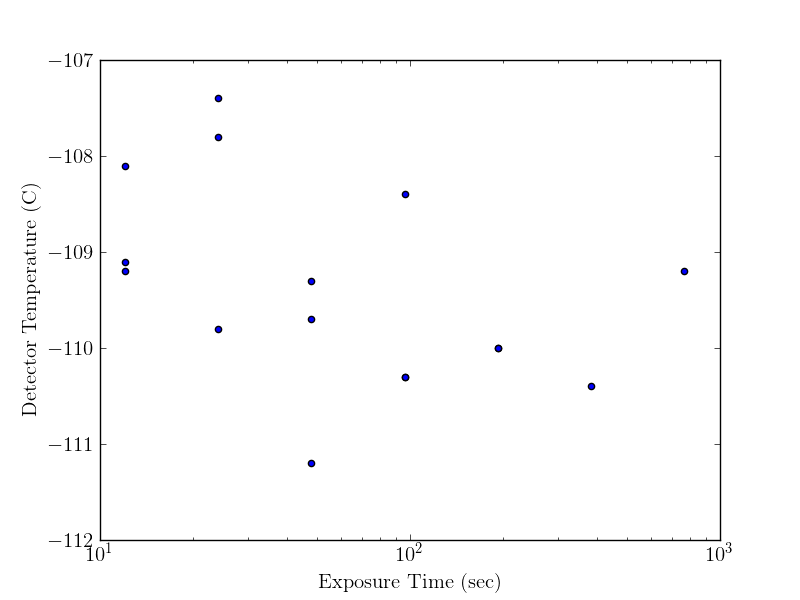
\includegraphics[width=.48\linewidth]{plots/exposure_temp.png}
\caption{Temperature of the CCD detector for different exposure frames does not vary more than about 4C.} \label{fig:temp}
\end{center}
\end{figure}

% ==================================
\section{Conclusion}
In conclusion we measure the gain of our detector to be about 0.31 ADU/electron and readnoise to be 34 electrons. For varied exposure times we find that the Poisson distribution applies better when the frequency of our counts are low, and the Gaussian distribution applies better when the frequencies are high. We also find that adding more data decreases the standard deviation of the mean by 1/$\sqrt{n}$. In the future, understanding the fundamental sources of noise and their statistics will allow us to determine what signals are significant in an observation and make meaningful scientific conclusions.

% ==================================
\section{Author Contributions}

This project was done in collaboration with Julian Beas-Gonzalez and Russell Van-Linge (Group E), using data collected by Group B. Russell wrote code for fitting Poisson and Gaussian distribtions and computing MOM/SDOM, Julian wrote code for histograms and computing MOM/SDOM, and I wrote code for combining frames/bias subtracting images, plotting histograms/images and slicing images (except for a few snippets for making histograms and reading fits files from the class notes). We met several times outside of class to compare results, fix issues, and combine our code together, which can be found on github: \href{https://github.com/jbirky/photonCounting}{https://github.com/jbirky/photonCounting}.

\begin{figure}[H]
\plotone{plots/exposure3.png}
\plotone{plots/exposure6.png}
\plotone{plots/exposure12.png}
\plotone{plots/exposure48.png}
\caption{Combined, bias-subtracted, flat frame histograms and images for varying exposure times (0, 3, 6, and 12 sec). \label{fig:flats1}}
\end{figure}
\begin{figure}[H]
\plotone{plots/exposure96.png}
\plotone{plots/exposure192.png}
\plotone{plots/exposure384.png}
\plotone{plots/exposure768.png}
\caption{Combined, bias-subtracted, flat frame histograms and images for varying exposure times (96, 192, 384, and 768 sec). \label{fig:flats2}}
\end{figure}

% ==================================
\newpage
\section{Appendix}

\lstset{language=Python,
        basicstyle=\footnotesize\ttfamily,
        keywordstyle=\color{blue},
        numbers=left,
        numberstyle=\ttfamily,
        stringstyle=\color{red},
        commentstyle=\color{gcolor},
        morecomment=[l][\color{gray}]{\#}
}

\subsection{Statistical Code} \label{code:stats}
\small
\hrule
\begin{lstlisting}
def mean(array):
    return np.sum(array)/len(array)

def stdev(array):
    return np.sqrt(sum((array - mean(array))**2)/(len(array) - 1))

def poisson_approx(data, mean):
    pdist = np.array(np.exp((data*np.log(mean))-(data*np.log(data))+data-mean))
    return pdist

def gaussian(data,mean,sigma):
    gdist = np.array((1/(sigma*(2*math.pi)**(.5)))*np.exp(-.5*((data-mean)/sigma)**2)) 
    return gdist
\end{lstlisting}
\hrule \vspace{7pt}

\subsection{Data Processing code} \label{code:data} 
\hrule
\begin{lstlisting}
def readData(folder):
    """
    Read all frames from a given directory into one matrix.
    input:  directory to folder containing frames
    output: array3d (dimension: xpixel x ypixel x # frames)
            array2D (dimension: 1D flattened img x # frames)
    """
    
    files = os.listdir(folder)

    array3D, array2D = [], []
    for ff in files:
        arr = fits.getdata(folder + ff)
        array3D.append(arr)
        array2D.append(arr.flatten())
    
    return np.array(array3D)

def combineFrame(data_array):
    """
    Combine image frames and return 1D array.
    input:  data array (dimension: # 1D detector counts x # frames)
    output: 1D combined array of detector counts (ADU)
    """
    
    return np.median(data_array, axis=0)
\end{lstlisting}
\hrule \vspace{7pt}

\subsection{Histogram/Image code} \label{code:plots} 
\hrule
\begin{lstlisting}
def plotAll(array2D, **kwargs):
    
    arr = array2D.flatten()
    
    avg = mean(arr)
    std = stdev(arr)
    med = np.median(arr)
    Npix = len(arr)    
    
    sigma = kwargs.get('sigma', 2)
    low = int(np.round((avg-sigma*std)))
    high = int(np.round((avg+sigma*std)))
    rng = kwargs.get('rng', [low, high])
    exp = kwargs.get('exp')
    if 'nbins' in kwargs:
        nbins = kwargs.get('nbins')
        bin_size = (rng[1]-rng[0])/nbins
    else:
        bin_size = kwargs.get('bin_size', 1)
    
    fig, (ax1, ax2) = plt.subplots(1,2, figsize=[18,6])
    
    # Histogram
    #===========
    hr = np.arange(rng[0], rng[1]+1, bin_size)
    hist = []
    for i in range(len(hr)):
        try:
            counts = len(np.where((arr >= hr[i]) & (arr < hr[i+1]))[0])
        except:
            counts = 0
        hist.append(counts)
    ax1.step(hr, hist, color='k')

    #mean and median lines
    ax1.axvline(avg, color='b', label=r'$\bar{x}=%s$'%(np.round(avg,2)))
    
    #sigma levels
    if kwargs.get('show_level', True) == True:
        for i in np.arange(1,sigma+1):
            if i == 1:
                ax1.axvspan(avg-i*std, avg+i*std, facecolor='g', alpha=0.05, \
                    label=r'$s=\pm %s$'%(np.round(std,2)))
            else:
                ax1.axvspan(avg-i*std, avg+i*std, facecolor='g', alpha=0.05)
                
                
    #poisson distribution
    xarray = np.arange(rng[0]-10, rng[1]+10, 1)
    pdist = poisson_approx(xarray, avg)
    pdist = max(hist)/max(pdist)*pdist
    ax1.plot(xarray, pdist, color='r', label=r'$P_{Poisson}(\bar{x})$')
    std_expected = math.sqrt(avg)
    ax1.axvspan(avg - std_expected, avg + std_expected, facecolor='r', alpha=0.05, \
                label=r'$\sigma=\pm %s$'%(np.round(std_expected,2)))
    
    #gaussian distribution
    gdist = gaussian(xarray, avg, std)
    gdist = max(hist)/max(gdist)*gdist
    ax1.plot(xarray, gdist, color='c', label=r'$P_{Gaussian}(\bar{x}, s)$')
    
    ax1.legend(loc='upper left')
    ax1.set_xlabel('Counts (ADU)')
    ax1.set_ylabel('Frequency')
    
    if 'exp' in kwargs:
        ax1.set_title('Combined Histogram (Exposure Time: %s sec)'%(exp))
    ax1.set_xlim(rng)
    
    # Image
    #===========
    hrng = kwargs.get('hrng', [np.percentile(arr, 10), np.percentile(arr, 90)])
    pl = ax2.imshow(array2D, origin='lower', interpolation='nearest', \
         cmap='gray', vmin=hrng[0], vmax=hrng[1])
    fig.colorbar(pl, ax=ax2, fraction=0.046, \
                 pad=0.04).set_label('Detector Value (ADU)')
    
    ax2.set_xlabel('pixels(x)')
    ax2.set_ylabel('pixels(y)')
    ax2.set_title('Combined Image')
    
    if 'save_dir' in kwargs:
        save_dir = kwargs.get('save_dir')
        plt.savefig(save_dir + 'exposure%s.png'%(exp))
    plt.show()
\end{lstlisting}
\hrule \vspace{7pt}

\subsection{Data Reduction} \label{code:reduction} 
\hrule
\begin{lstlisting}
files = natsorted(os.listdir('data/'))[1:]
exp_times = np.array([int(f.split('exp')[1]) for f in files])

#combined frames, and combined frames in counts per second
counts, counts_ps = [], []
for exp in exp_times:
    
    #Read frames, subtract combined bias, combine frames
    array3D = readData('data/exp%s/'%(exp))
    bias_sub_3D = [(frame - bias_2D) for frame in array3D]
    array2D = combineFrame(bias_sub_3D)
    
    array2D_cps = array2D/exp
    
    #cut out safe part of image
    cut = Cutout2D(array2D, window[0], window[1]).data
    cut_cps = Cutout2D(array2D_cps, window[0], window[1]).data
    
    counts.append(cut.flatten())
    counts_ps.append(cut_cps.flatten())
    
    #Plot histogram and image & save to .png
    plotAll(cut, sigma=3, exp=exp, show_level=True, save_dir='writeup/plots/')
\end{lstlisting}
\hrule \vspace{7pt}

\subsection{Gain Calculation} \label{code:gain} 
\hrule
\begin{lstlisting}
xbar = np.mean(counts, axis=1)
s = np.std(counts, axis=1)

#fit polynomial
x_arr = np.arange(0, 10**5, 10**2)
fit = np.polyfit(xbar, s**2, 2)
y_arr = np.polyval(fit, x_arr)
\end{lstlisting}
\hrule \vspace{7pt}

\subsection{MOM and SDOM Calculation} \label{code:mom_sdom} 
\hrule
\begin{lstlisting}
files = np.array(natsorted(os.listdir()))
data = []

# Go through each frame, take the median, subtract bias, and divide 
# by exposure time
for i in files:

    # loading in the data
    frame_data = fits.getdata(i)
    frame_exp = fits.open(i)
    exp_time = frame_exp[0].header['EXPTIME']
    # Subtracting the bias
    data_subbed = frame_data - bias_2D
    data_median_ps = np.median(data_subbed,axis=0)/exp_time
    # Median of each frame divided by exposure time for that frame
    data.append(data_median_ps)
   
data = np.array(data)

# Setting up arrays 
mom = []
std = []
num_frame = np.arange(2,len(data)+1)

# Calculates MOM and SDOM 
i = 2
while i < len(data)+1:
    frames = data[:i]
    mean = np.mean(frames) 
    stand = np.std(frames)
    mom.append(mean)
    std.append(stand)
    i = i + 1

plt.scatter(num_frame,mom,marker='x',color='black',label='MOM')
plt.scatter(num_frame,std,marker='v',color='gray',label='SDOM')
plt.show()
\end{lstlisting}
\hrule \vspace{7pt}

% \lstinputlisting[language=Matlab]{./Code/calc_error.m}

% \begin{thebibliography}{}
% \bibitem[Astropy Collaboration et al.(2013)]{2013A&A...558A..33A} Astropy Collaboration, Robitaille, T.~P., Tollerud, E.~J., et al.\ 2013, \aap, 558, A33 
% \end{thebibliography}


\end{document}

